\input{boilerplate}
\begin{document}
\bibliographystyle{unsrt}

\title{High-resolution 7-Tesla fMRI data on the perception of musical genres -- an extension to the studyforrest dataset}

\author[1,2]{Michael~Hanke}
\author[1]{Richard~Dinga}
\author[1]{Christian~Häusler}
\author[3]{J.~Swaroop~Guntupalli}
\author[1,4]{Falko~R.~Kaulke}
\author[5]{J\"org~Stadler}

\affil[1]{Psychoinformatics lab, Department of Psychology II, University of
Magdeburg, Magdeburg, Germany}
\affil[2]{Center for Behavioral Brain Sciences, Magdeburg, Germany}
\affil[3]{Department of Psychological and Brain Sciences,
  Dartmouth College, Hanover, New Hampshire, USA}
\affil[4]{Visual Processing Laboratory, Ophthalmic Department,
Otto-von-Guericke-University, Magdeburg, Germany}
\affil[5]{Leibniz Institute for Neurobiology, Magdeburg, Germany}
\maketitle
\thispagestyle{fancy}

\begin{abstract}
% Abstracts should be up to 300 words and provide a succinct summary of the
% article. Although the abstract should explain why the article might be
% interesting, care should be taken not to inappropriately over-emphasise the
% importance of the work described in the article. Citations should not be used
% in the abstract, and the use of abbreviations should be minimized.
\hl{highlighted text indicates a TODO item}
\end{abstract}
\clearpage

\section*{Background}
%The format of the main body of the article is flexible: it should be concise
%and in the format most appropriate to displaying the content of the article.

%A brief summary of how this work was motivated and how it links to existing
%and future work.
audio movie has lots of music

studying music perception in a complex stimulus becomes easier if there is a simpler reference

this is the reference

\cite{CTK+2012}

The complexity of the different kind of music (spectra, depth, preference etc.)  contribute to differnet state of minds which can be analysis separately, especially in connection with (more detailed) annotions of the movie or different ROI based analyses.

\subsection*{Possible applications}

\section*{Materials and methods}
\subsection*{Participants}

Acquisition of the data described herein was part of a previously published
study \cite{HBI+14}, and took place in close temporal proximity (no more
than a few weeks apart). The participants in this data release are identical to
those previously reported \cite{HBI+14}.  They were fully instructed about
the nature of the study and were paid a total of \unit[100]{EUR} for their
participation, which included the previously reported data acquisitions, as
well as the one described herein. All data acquisitions were jointly approved
by the ethics committee of the Otto-von-Guericke-University of Magdeburg,
Germany.


\subsection*{Stimulus}

All stimuli employed in this study are identical to those used in a previous
study \cite[for details refer to][]{CTK+2012}. They were five natural,
stereo, high-quality music stimuli for each of five different musical genres:
1) Ambient, 2) Roots Country 3) Heavy Metal, 4) 50s Rock'n'Roll, and 5)
Symphonic.  Each stimulus was a six second excerpt from the center of each
musical piece \hl{Is the piece really at the center?}.  Excerpts were normalized so that their RMS values were equal,
and a \unit[50]{ms} quarter-sine ramp was applied at the start and end of each excerpt
to suppress transients.


\begin{figure*}
  \centering
  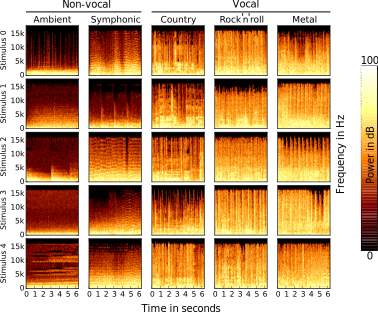
\includegraphics[width=\linewidth]{stimulus_specgrams}\\
  \caption{Spectrogram.}
  \label{fig:spectrograms}
\end{figure*}


\subsection*{Procedures and stimulation setup}

The setup for audio-visual presentation was as previously reported
\cite{HBI+14}. Participants listened to the audio using custom-built in-ear
headphones that were driven by an MR confon mkII+ fed from an Aureon 7.1 USB
(Terratec) sound card through an optical connection.
Visual instructions were presented with an LCD projector (DLA-G150CL, JVC Ltd.)
on a rear-projection screen positioned behind the head coil within the magnetic
bore. Participants viewed the screen through a mirror attached to the head
coil.

At the start of each recording session, during the preparatory MR scans,
participants listened to a series of longer excerpts of musical pieces and
songs from the five different genres. During this phase participants were
instructed to request adjustments of the stimulus volume in order to guarantee
optimal perception of the stimuli against the noise pedestal emitted by the
scanner. There was no overlap between the songs presented in this phase and those
used as stimuli in the main experiment.

Eight scanning runs followed the initial sound calibration. Each run was
started by the participant with a key-press ready signal. Each run comprised 25
trials, five stimuli for each of the five genres. These 25 stimuli were identical
across runs and presented exactly once per run. The onset of each stimulus was
synchronized with the volume acquisition trigger signal emitted by the scanner.
Order of stimulus genres within each run was counter-balanced using De Bruijn
cycles \cite{AMM+2011} (alphabet size = 5, counter-balancing level = 2),
hence each genre was followed by any other genre equally often and exactly
once.  For each of the eight runs a unique De Bruijn cycle was generated.
However, the same set of 8 cycles was used for all participants in the study,
while randomizing the order of run sequences across participants. This was done
in order to maintain synchronous stimulation across participants for the
application of the hyperalignment algorithm \cite{HGC+11}. At the end of each run
participants were given the opportunity for a break of variable length until
the indicated readiness for the next run. Most participants started the next
run within a minute.

Each run started with a white fixation cross in the center of the screen. With
the beginning of each trial, synchronous with the start of the stimulus, the
fixation cross turned green to indicated music playback, and changed back to
white after the playback had stopped.  In order to further disentangle
responses to individual genres, each trial was followed by a variable delay of
4, 6, or 8 seconds. For each of the five trials for any given genre, the 4 and
8 second delay occurred once, while the remained three trials had a 6 second
delay period. The order of delay lengths was randomized within a run's
stimulation sequence. During trials with an 8 second delay subjects were
presented with a yes/no question that replaced the fixation cross four seconds
after the end of the music stimulus. The content of the question was randomized
and asked for particular features of the stimulus that had just ended (``Was
there a female singer?'', ``Did the song have a happy melody?'', etc.).
Participants had to indicated their response by pressing one of two buttons
with the index or middle finger of their right hand corresponding to the
response alternative presented on the screen. ``Yes'' was always mapped to the
left side (index finger), ``No'' always to the right side (middle finger).  The
question had the purpose of keeping the participants attentive to the stimuli and
counteract the affect of increasing familiarity across multiple runs.  This
stimulation procedure guaranteed a minimum of four seconds of uniform
stimulation (no audio stimulus, no visual stimulus other than a white fixation
cross) after each musical stimulus.

Stimulus presentation and response logging were implemented using PsychoPy
\cite{Pie2007}.  The source code of the complete implementation of the experiment, as
well as the actual stimulus sequences used for each run are available as
Supplementary Material in the data release. PsychoPy was running on a computer
with the (Neuro)Debian operating system \cite{HH12}.

\subsection*{Functional MRI data acquisition}

The acquisition protocol for functional MRI was largely identical with the one
previously reported \cite{HBI+14}, hence only differences and key facts are
listed here.

Importantly, the same landmark-based procedure for automatic slice positioning
that was used to align the scanner field-of-view between acquisition sessions,
was used again to align the field-of-view for this acquisition with the one in
the previous study \cite{HBI+14}. As the exact same alignment target was
used, this led to a very similar field-of-view configuration across
acquisitions.

Each acquisition run consisted of 153 volumes (repetition time of 2.0 seconds
with no inter-volume gaps), for a total of eight runs. All functional MRI data
were converted from the DICOM format into the NIfTI format for publication.
Furthermore, following a de-identification procedure described elsewhere
\cite{HBI+14} voxels in the vicinity of facial features, auricles, or teeth
were zeroed out in the published images. Binary mask images indicating which
voxels were altered are provided.

\subsection*{Physiological recordings}

The cardiac and respiratory trace was recorded for the full duration of all
eight runs. The acquisition setup for physiological was identical with the one
previously reported \cite{HBI+14}.

\subsection*{Dataset content}

The released data comprises\ldots

\paragraph{Source code}

The full source code for all descriptive statistics and figures included in
this paper is available\ldots

\section*{Dataset validation}
%Use section and subsection commands to organize your document. \LaTeX{}
%handles all the formatting and numbering automatically. Use ref and label
%commands for cross-references.

%This section is not essential for Web Tool papers.
%For Data Articles, no analysis of the data, results or conclusions should be
%included and so this section should not be completed.

predict music segment, as given as example in introduction

MOTION FIGURE


\begin{table}
  \centering
  \caption{Overview of known data anomalies (F: functional data,
    P: physiological recordings during fMRI session)}
  {\renewcommand{\arraystretch}{1.2}
  \begin{tabular}{lllp{9cm}}
    \toprule
    Modality & Participant & Run & Description \\
    \midrule
    F \& P & 20 & 5-8 & no data; participant aborted experiment after four runs \\
    \bottomrule
  \end{tabular}
}
  \label{tab:anomalies}
\end{table}


\section*{Data availability}

\texttt{This section will be auto-generated.}


\section*{Consent}

Written informed consent for publication of acquired data in a de-identified
form was obtained from all participants.

\section*{Author contributions}
%In order to give appropriate credit to each author of an article, the
%individual contributions of each author to the manuscript should be detailed
%in this section. We recommend using author initials and then stating briefly
%how they contributed.

MH conducted the study, implemented the stimulation paradigm, performed dataset validation analysis, and wrote the manuscript.
RD implemented and performed the dataset validation analyses.
CH converted the stimulation protocol into the OpenFMRI format.
JSG contributed to the implementation of the stimulation paradigm, and contributed to the validation analysis.
JS was the data acquisition lead.

\section*{Competing Interests}
No competing interests were disclosed.

\section*{Grant Information}

This research was supported by the German Federal Ministry of Education and
Research (BMBF) as part of a US-German collaboration in computational
neuroscience (CRCNS; awarded to James Haxby, Peter Ramadge, and Michael Hanke),
co-funded by the BMBF and the US National Science Foundation (BMBF 01GQ1112;
NSF 1129855). Michael Hanke was supported by funds from the German federal
state of Saxony-Anhalt, Project: Center for Behavioral Brain Sciences.

\section*{Acknowledgements}
%This section should acknowledge anyone who contributed to the research or the
%article but who does not qualify as an author based on the criteria provided
%earlier (e.g. someone or an organisation that provided writing assistance).
%Please state how they contributed; authors should obtain permission to
%acknowledge from all those mentioned in the Acknowledgements section.  Please
%do not list grant funding in this section (this should be included in the
%Grant information section - See above).

We are grateful to Andr\'e Brechmann for his feedback on the results of the
classification analysis.

{\small
  \bibliography{references}
}%\small
\end{document}

% vim: textwidth=80 colorcolumn=81
